% Appendix D, Figure D.2 --- "The octahedral POVM, end to end".  The layout only.
%
% THIS FILE IS THE TEMPLATE.  The other four card bodies declare this header
% binding and list only their own deviations.  Every rule below was bought with
% a measurement in the real class (11pt scrbook, a4paper, margin=1in,
% \textwidth 452.9679pt, \textheight 700.50687pt); do not "tidy" any of them.
%
% WHAT A CARD IS.  The card labels rather than narrates: a header strip the
% reader has already met in Figure 1.1, four objects, one label per object,
% and a pointer per band.  The strip is Figure 1.1's own \RecipeSeriesStrip --
% its column heads and this solid's row, character for character, minus the
% name column -- plus one spanned footer carrying the thesis's exactness
% conjunction in nine words.  That is what makes the recognition a build
% check (assertion 30) rather than a hope.
%
% Everything numeric comes from ../code/data/card_oct_data.tex, which
% code/_build_povm_cards.py writes after its checks against the npz data,
% Decker's circuits as randomized_decker rebuilds them, Figure 1.1's own
% recipe_tet_data.tex, and Tables E.1, 5.2, D.1, D.3 and D.4 -- and refuses to
% write a byte if any of them fails.  The heads, the labels and the caption are
% emitted too, so this file holds the LAYOUT and nothing else; assertion 12
% requires the facts on the page verbatim and assertion 29 parses the printed
% surface back out of the data file, cell by cell.
%
% The four numerals must read 1..4 straight down the left edge.
%
% ASSEMBLY RULES (each one bought with a measurement; do not "tidy" them):
%   * rows are stacked in one \vbox and separated by \vskip<n>pt\nointerlineskip,
%     and EVERY source line inside the \vbox ends in %.  Without either, LaTeX
%     adds ~13.6pt of baseline glue PER ROW: the same dodecahedron body measured
%     726.79pt with the glue and 662.96pt without.
%   * the body is a plain \vbox, NEVER \vbox to.  Equal-height bodies were
%     measured and rejected: they strand the tetrahedron's caption 152pt below
%     its own content.  The five start at the same height because the float
%     pages are top-aligned locally (bsc-thesis.tex brackets these five floats
%     with \@fptop 0pt and restores the default after the \clearpage); ragged
%     bottoms, aligned tops.
%   * a two-column row is one \hbox to \hsize{<left>\hfil<right>} whose columns
%     are \vtop's opening with \hbox{}\nointerlineskip, which is what top-aligns
%     them (a \vtop otherwise aligns on its first line's baseline).
%   * every prose block is \PBOX: \sloppy plus \emergencystretch, or the
%     unbreakable math atoms throw overfull boxes into the neighbouring column.
%     WIDEN A COLUMN BY 4pt BEFORE TOUCHING A SENTENCE.
%   * NOTHING may be glued to the right of the U_R atom.  At \footnotesize this
%     card's product measured 181.64pt bare and 190.89pt with an em-dash
%     attached, a 3.58pt overfull box.  Every rider therefore follows the
%     CLAUSE, never the formula, and the generator's params() carries the note.
%   * the parameter block is ONE FORMULA PER LINE (\par\vskip1pt between), full
%     width, at \small.  Set as a justified paragraph at \footnotesize, the
%     inline 4x4 A opens a four-line hole; A belongs to the chapter head
%     (assertion 32) and the block reads as a list.  Justified, not
%     \raggedright: \raggedright costs +12.69pt.
%   * the vertex table and the key are set flush RIGHT in their columns; the
%     circuit is set flush LEFT, never centred, because all 13.73bp of xy-pic's
%     slack is on the right and centring hangs the \lstick ket bar into the
%     left margin.
%   * FOUR band rules, one per band, \vskip2pt\hrule height0.5pt\vskip1.5pt =
%     4.00pt each.  No other rules, no boxes, no tints, NO COLOUR: the
%     numbered chips do identity, so the pages are greyscale-safe.
%   * every head must fit on ONE line with its pointer.  Measured natural
%     widths against the 452.9679pt line: head 2 with its pointers is 348.82
%     on all five, and head 4 is the tightest at 437.53 on the A_5 pair
%     (", rightmost factor first" + three pointers, 15.44pt of slack).
%     Re-measure before rewording any head or giving a band a fourth pointer;
%     the strip and the dodecahedron's ray list may not change without
%     re-measuring either (the ray list is 443.86pt natural -- 9.11pt of
%     slack).
%   * \PanelScale 2.47 on all five, Figure 1.1's own.  The tetrahedron reuses
%     Figure 1.1's recipe_tet_sphere.pdf byte for byte, not redrawn.
%   * the float, not the body, is what LaTeX measures: \@largefloatcheck
%     compares \ht\@currbox against \textheight = 700.50687pt.  Measure over
%     the FLOAT: a pass over the body alone leaves the kappa label's \cite
%     unresolved -- no biber -- and inflates.  Measured that way, with
%     bsc-thesis.aux's labels replayed and biber run, the five reserves are
%     tet 171.63pt, oct 90.35, cube 35.99, icos 56.01, dodec 21.30; a card
%     that takes an extra band-4 line pays about 11pt of its reserve for it.
%   * the caption is ONE line on all five and must stay one: a second line
%     costs 13.60pt against the dodecahedron's 21.30pt of reserve.  Measured
%     with \@makecaption in this class: the shipped caption sets 429.82pt
%     (Fig.~7) / 435.29pt (Figs.~11 and~13) WITH its "Figure D.5.: " label,
%     against the 452.9679pt line, and the caption box is 23.60pt with 0
%     overfull.  A longer wording that also calls the $U_g$ box dashed
%     ("$U_R$ and the dashed $U_g$ are ours") measures
%     485.24 / 490.71pt and does NOT break: \@makecaption still returns a
%     23.60pt box and TeX reports Overfull \hbox 9.07 / 14.55pt.  Head 2
%     names the dashed box one band above, which is what pays for the cut.
%   * THE DODECAHEDRON IS THE BINDING CARD, at 21.30pt of reserve.  Every
%     literal in the generator's emitters is shared, so any wording change
%     must be re-measured against card_dodec_body.tex before it ships.  Two
%     of its objects are already at the edge: the kappa label (its box must
%     stay near the 75.56pt key) and the U_R parameter line (one word of
%     rider wraps it: "twirls the noise" measures 490.81pt against the
%     452.9679pt line; "twirls" ships at 448.53).  Its ray line is 443.86pt
%     natural -- 9.11pt of slack.
%   * ... but one shared literal binds its WIDTH elsewhere: the
%     M-tilde-dagger line's gloss, ", the Naimark extension unitary the solid
%     box implements".  The tetrahedron prints the longest of the five
%     formulas, so the gloss sets 438.23pt there against 351.56 on the
%     dodecahedron -- 14.73pt of slack, and "the boxed circuit" in place of
%     "the solid box" misses by 3.02pt and wraps.
%
% WORDING RULES:
%   * print the positive with the negative.  The strip's spanned footer carries
%     the conjunction on every card -- "only the octahedral coin is exact ---
%     this dilation is not" -- with the negative also in the `reorientation
%     exact?` cell beside it; on this card the positive is its own row's
%     `3 axes --- exact`.  The dilation clause is what binds Theorem 1 to the
%     circuit printed 10cm below it and may not be compressed away.  Its
%     polarity is fragile: "exact, this dilation included" reads as putting
%     the dilation AMONG the exact things -- the appositive needs the host
%     Figure 1.1 gives it ("any dilation, this one included") -- so this card
%     spells the negative out instead.
%   * Decker is named WITH the cite wherever his objects appear: the caption
%     (the solid box) and the kappa label (his own outcome list).  Figure 1.1
%     prints no cold names; the cards do the opposite -- a \cite for
%     everything belonging to Decker, and his name with it.
%   * say what a reorientation IS before asking whether it is exact -- the
%     chapter head does it one page earlier, in its second sentence, and the
%     strip's head is Figure 1.1's own `reorientation exact?`.
%   * the two randomized protocols stay distinct.  "coin over axes" is
%     Figure 1.1's hyperlinked phrase, in the strip and in head 4; the twirl
%     appears as "a drawn $U_g$ twirls and relabels outcomes by $g^{-1}$" on
%     the parameter line, as "the drawn twirl" in the kappa label, and on the
%     tetrahedron as the contrast in band 4.  Every card's protocol line
%     closes with its own DRAW NOTE, the five together a ladder: no
%     projective route at all (the tetrahedron, where drawing anyway
%     assembles the cube), the twirl binding on this card and the cube
%     (realization needs only the three or four words printed above the
%     sentence), the two meeting at the icosahedron (the two-jobs sentence,
%     still that card's alone), realization binding on the dodecahedron.
%     Check 19d derives all five and pins each phrase to its own card: the
%     two-jobs one here would contradict the thesis's own counterexample,
%     this card's coin realizing and twirling nothing.  Head 4's "no ancilla"
%     is what says the coin REPLACES the dilation rather than running inside
%     it -- neither Figure 1.1 (which never explains the coin) nor the
%     protocol line supplies that, and it negates the strip's own `anc.` cell
%     two bands above, so it costs no new noun.
%   * direction is g^{-1}.  Never "acts on" -- assertion 11 greps this file.
%   * no italic run-in heads.
%   * the register convention lives ON THE OBJECT: the key rectangle's `upper`
%     stub and `lower` spanned head, whose bit widths say which wires those
%     are, plus head 3's "top wire first".
%   * one page, two F's: the circuit's upright sans $\mathsf F_3^\dagger$ and
%     band 4's bold $\mathbf F$ are different objects a band apart.  Never
%     gloss $\mathbf F = \mathbf H\mathbf S^\dagger$ here.
%   * the coin's order is the drawn word FIRST, the fixed alignment after it,
%     and the alignment is a LABEL, not a sentence ("($\Id$ here)").  Assertion
%     19b builds the reversed order and requires it to miss the vertex set.
%
% All macros below are \def and therefore local to the figure environment.
\parindent=0pt \parskip=0pt
% Auto-generated by code/_build_povm_cards.py -- DO NOT EDIT.
% The data blocks of the octahedral card of Appendix D
% (paper/figures/card_oct_body.tex \input's this and calls them).  Every
% number is derived from code/data/*.npz, Decker's circuits as
% randomized_decker rebuilds them, Figure 1.1's own \RecipeSeriesStrip, and
% Tables E.1, 5.2, D.1, D.3 and D.4, and is checked back against them before
% this file is written; see the builder's docstring for the checks (and
% _povm_cards_controls.py, which shows each of them failing on one corrupted
% literal: 100 negative controls, all aborting, 0 stale).
% Requires: booktabs, mathtools, hyperref, and the thesis macros \Id, \pmat,
% \bra, \ket, \braket, \Tr, \C, \sigmavec, \TwoT, \TwoO, \TwoI, \phig,
% \invphig, \sigmaz.  The body defines \NIS, \CTR, \PBOX, \COL, \FULLHEAD,
% \BANDRULE and \TAB, which \CardSide and the tables use.
% Regenerate with `cd code && uv run _build_povm_cards.py`.

\newcommand{\CTitle}{The octahedral POVM, end to end}
\newcommand{\CPtrStrip}{Introduction reference: Figure~\ref{fig:tetrahedron-recipe}}
\newcommand{\CHeadA}{Vertices and effects, $E_k = \tfrac1V(\Id + \hat n_k \cdot \sigmavec)$.}
\newcommand{\CPtrA}{Table~\ref{tab:povm-atlas} $\cdot$ Equation~\eqref{eq:povmform}}
\newcommand{\CHeadB}{Circuit; the dashed $U_g$ is an optional prepended rotation.}
\newcommand{\CPtrB}{Section~\ref{subsec:rotated-povms} $\cdot$ Table~\ref{tab:decker-pose}}
\newcommand{\CHeadC}{Register $\to$ vertex, top wire first; --- never fires}
\newcommand{\CPtrC}{Table~\ref{tab:decker-labels} $\cdot$ Section~\ref{sec:decker:using}}
\newcommand{\CHeadD}{Coin over axes, no ancilla, $\ket0$-vertex first}
\newcommand{\CPtrD}{Table~\ref{tab:decker-vs-coin} $\cdot$ Section~\ref{subsec:randomized-implementations} $\cdot$ Table~\ref{tab:binary-octahedral-group-2o}}

\newcommand{\CStrip}{{\footnotesize\setlength{\tabcolsep}{4pt}\renewcommand{\arraystretch}{0.88}%
\begin{tabular}{@{}c c c c l l l@{}}
\toprule
$V$ & group & anc. & dead & reorientation exact? & relabelling & \hyperref[tab:decker-vs-coin]{coin over axes}\\
\midrule
6 & $\TwoO$ & 2 & 2 & no thesis gate set & permuted & 3 axes --- \textbf{exact}\\
\midrule
\multicolumn{7}{@{}l@{}}{only the octahedral coin is exact --- this dilation is not (Theorem~\ref{thm:main}, Appendix~\ref{sec:decker:exactness})}\\
\bottomrule
\end{tabular}}}

\newcommand{\CardVertexTable}{%
\begin{tabular}{@{}r l c r@{}}
\toprule
$k$ & $\hat n_k$ & $E_k\ (\times\tfrac16)$ & $\bra{0}E_k\ket{0}$ \\
\midrule
$1$ & $(+1,\,\phantom{+}0,\,\phantom{+}0)$ & $\pmat{1 & 1 \\ 1 & 1}$ & $0.1667$ \\ \addlinespace[3pt]
$2$ & $(-1,\,\phantom{+}0,\,\phantom{+}0)$ & $\pmat{1 & -1 \\ -1 & 1}$ & $0.1667$ \\ \addlinespace[3pt]
$3$ & $(\phantom{+}0,\,+1,\,\phantom{+}0)$ & $\pmat{1 & -i \\ i & 1}$ & $0.1667$ \\ \addlinespace[3pt]
$4$ & $(\phantom{+}0,\,-1,\,\phantom{+}0)$ & $\pmat{1 & i \\ -i & 1}$ & $0.1667$ \\ \addlinespace[3pt]
$5$ & $(\phantom{+}0,\,\phantom{+}0,\,+1)$ & $\pmat{2 & 0 \\ 0 & 0}$ & $0.3333$ \\ \addlinespace[3pt]
$6$ & $(\phantom{+}0,\,\phantom{+}0,\,-1)$ & $\pmat{0 & 0 \\ 0 & 2}$ & $0.0000$ \\ \addlinespace[3pt]
\bottomrule
\end{tabular}
}

\newcommand{\CIdent}{$\sum_k E_k = \Id$, $\Tr E_k = \tfrac13$, rank one, a $3$-design; the Pauli eigenprojectors, $\times\tfrac13$.}
\newcommand{\CIdentB}{}

\newcommand{\CParams}{$U_R = R_{\hat z}(180^\circ)R_{\hat y}(-\arccos(1/\sqrt3))R_{\hat z}(-45^\circ)$, rightmost factor first, inverts Table~\ref{tab:decker-pose}'s $R$; a drawn $U_g$ twirls and relabels outcomes by $g^{-1}$.\par\vskip1pt $Q_8^\dagger$: the CNOT $\ket{000}\mapsto\ket{000}$, $\ket{101}\mapsto\ket{001}$; $\mathsf{F}_3^\dagger \oplus I_1 \in \C^{4\times4}$, lower two wires\par\vskip1pt $\tilde{M}^\dagger_8 = (U_A \otimes (\mathsf{F}_3^\dagger \oplus I_1))\,Q_8^\dagger$, the Naimark extension unitary the solid box implements}

\newcommand{\CardSide}{\CTR{\hsize}{$U_A = \sqrt3\,\pmat{\alpha & \beta \\ \beta & -\alpha}$}\NIS{4pt}\CTR{\hsize}{$\alpha = \sqrt{(3+\sqrt3)/18}$}\NIS{4pt}\CTR{\hsize}{$\beta = \sqrt{(3-\sqrt3)/18}$}}

\newcommand{\CardKey}{%
\begin{tabular}{@{}c c c c c@{}}
\toprule
& \multicolumn{4}{c}{\footnotesize lower} \\
{\footnotesize upper} & $\mathtt{00}$ & $\mathtt{01}$ & $\mathtt{10}$ & $\mathtt{11}$ \\
\midrule
$\mathtt{0}$ & 5 & 3 & 1 & --- \\
$\mathtt{1}$ & 6 & 4 & 2 & --- \\
\bottomrule
\end{tabular}
}

\newcommand{\CKappa}{Run $U_R$ and read the key, or skip $U_R$ and read Decker's own numbered list~\cite{decker2004quantumcircuitssinglequbit}: either way $\kappa = 1$, free. His circuit with our list, index for index, is the mismatch: $\kappa = +0.321975$; under the drawn twirl it costs a $1/\kappa^2 = 9.65\times$ premium in shots, never a bias.}

\newcommand{\CRays}{$\mathbf{F}^\dagger$~$1$,\,$2$ $\cdot$ $\mathbf{F}$~$3$,\,$4$ $\cdot$ $\Id$~$5$,\,$6$}

\newcommand{\CCoin}{Draw one, apply it, then the alignment ($\Id$ here); measure $Z$. Random Pauli measurement. Realization needs only these three; among groups it is the twirl that forces the full $\TwoT$ draw (Section~\ref{sec:shadows:bills}).}

\long\def\NIS#1{\vskip #1\nointerlineskip}
\long\def\CTR#1#2{\hbox to #1{\hss #2\hss}}
\long\def\PBOX#1#2{\vtop{\hsize=#1\parindent0pt\sloppy\emergencystretch=1.5em\small #2}}
\long\def\COL#1#2{\vtop{\hsize=#1\parindent0pt\hbox{}\nointerlineskip #2}}
\long\def\FULLHEAD#1#2#3{\hbox to \hsize{\small\textbf{#1}\,#2\hfil{\footnotesize #3}}}
\def\BANDRULE{\vskip2pt\hrule height0.5pt\vskip1.5pt\nointerlineskip}
\long\def\TAB#1{{\small\renewcommand{\arraystretch}{0.88}\setlength{\tabcolsep}{3pt}#1}}
%
\vbox{\hsize\textwidth\parindent0pt
%
% --- title and the header strip: Figure 1.1's own row -----------------------
\hbox to \hsize{\large\bfseries \CTitle\hfil{\normalfont\footnotesize \CPtrStrip}}%
\NIS{5pt}%
\hbox{\CStrip}%
\BANDRULE
%
% --- band 1: the object -----------------------------------------------------
% Where the effect table is the taller column, the sphere is vertically
% centred against it.  The offset is computed at TeX time from the two
% boxes, so a regenerated table cannot strand a hand-measured constant;
% the row's total height is unchanged (the taller column still sets it).
% The other three cards keep the template's top alignment -- their panels
% are the taller column.
\FULLHEAD{1}{\CHeadA}{\CPtrA}%
\NIS{5pt}%
\setbox0=\hbox{\TAB{\CardVertexTable}}%
\setbox2=\hbox{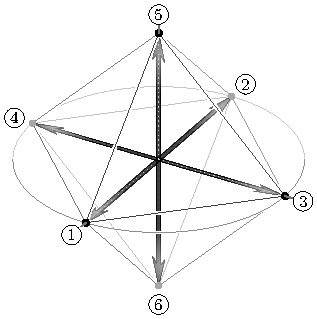
\includegraphics{figures/card_oct_sphere.pdf}}%
\dimen0=\dimexpr(\ht0+\dp0-\ht2-\dp2)/2\relax
\hbox to \hsize{%
  \COL{170pt}{\vskip\dimen0 \CTR{170pt}{\box2}}%
  \hfil
  \COL{277pt}{\hbox to 277pt{\hfil\box0}}%
}%
\NIS{4pt}%
\PBOX{\hsize}{\CIdent}%
\BANDRULE
%
% --- band 2: the machine ----------------------------------------------------
\FULLHEAD{2}{\CHeadB}{\CPtrB}%
\NIS{5pt}%
\hbox to \hsize{%
  \COL{264pt}{\hbox to 264pt{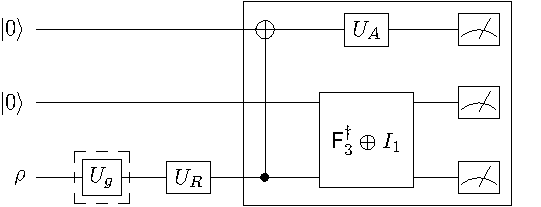
\includegraphics{figures/card_dec_oct.pdf}\hss}}%
  \hfil
  \COL{183pt}{\small\CardSide}%
}%
\NIS{5pt}%
\PBOX{\hsize}{\CParams}%
\BANDRULE
%
% --- band 3: the readout ----------------------------------------------------
\FULLHEAD{3}{\CHeadC}{\CPtrC}%
\NIS{5pt}%
\hbox to \hsize{%
  \COL{150pt}{\TAB{\CardKey}}%
  \hfil
  \COL{294pt}{\PBOX{294pt}{\CKappa}}%
}%
\BANDRULE
%
% --- band 4: the alternative ------------------------------------------------
\FULLHEAD{4}{\CHeadD}{\CPtrD}%
\NIS{5pt}%
\PBOX{\hsize}{\CRays}%
\NIS{2pt}%
\PBOX{\hsize}{\CCoin}%
}%
